\documentclass[tikz,border=1pt]{standalone}

\usepackage{amsmath}
\usepackage{xcolor}
\usepackage{tikz}
\usepackage{helvet}
\renewcommand{\familydefault}{\sfdefault}  % Set sans-serif as default

\usetikzlibrary{arrows.meta}
\usetikzlibrary{calc, fit, matrix, positioning}

\tikzstyle{circ}=[circle, draw, minimum size=1.2cm]
\tikzstyle{square}=[rectangle, draw, minimum size=1.2cm]

\begin{document}

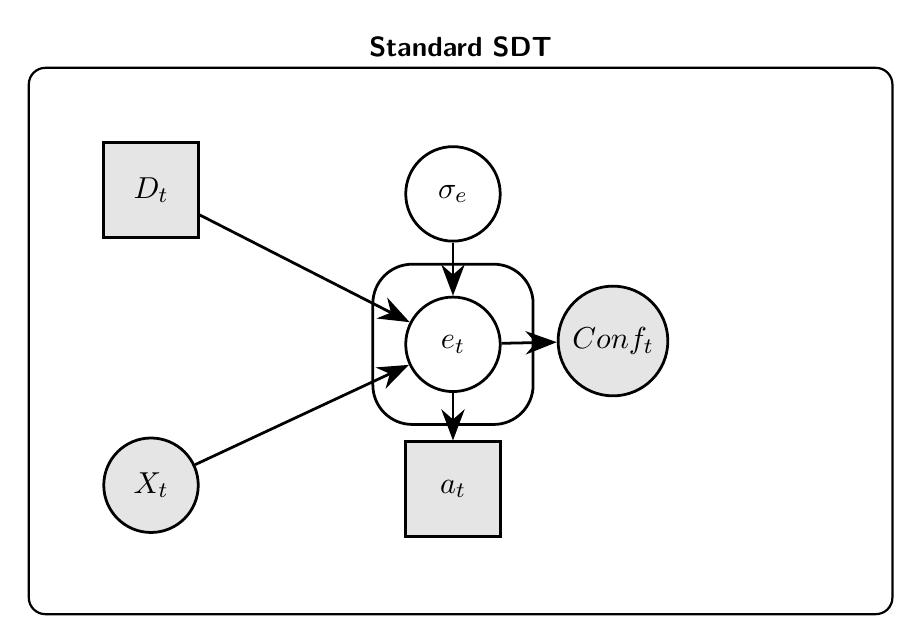
\begin{tikzpicture}

\tikzset{>={Stealth[scale=1.5]}}
\tikzset{every node/.style={font=\sffamily\fontsize{11pt}{12pt}\selectfont}}
\tikzset{every path/.style={line width=1pt}}

% Main matrix
\matrix (m0) [
    ampersand replacement=\&,
    matrix of math nodes,
    nodes in empty cells,
    column sep=.7cm,
    row sep=0.5cm,
]
{
    |[square, draw, fill=gray!20]| D_t \& 
    |[minimum size=1.2cm, inner sep=0pt, draw=none]| \& 
    |[circ, draw]| \sigma_e \&
    |[minimum size=1.2cm, inner sep=0pt, draw=none]| \\
    |[minimum size=1.2cm, inner sep=0pt, draw=none]| \&
    |[minimum size=1.2cm, inner sep=0pt, draw=none]| \&
    |[circ, draw]| e_t \&
    |[circ, draw, fill=gray!20]| Conf_t \&   \\
    |[circ, draw, fill=gray!20]| X_t \&
    |[minimum size=1.2cm, inner sep=0pt, draw=none]| \&
    |[square, draw, fill=gray!20]| a_t \& 
    |[minimum size=1.2cm, inner sep=0pt, draw=none]| \&
    |[minimum size=1.2cm, inner sep=0pt, draw=none]| \\
};

% Arrows for motor system and efference copy
\draw[->] (m0-1-3) -- (m0-2-3); % sigma -> e_t
\draw[->] (m0-1-1) -- (m0-2-3); % D_t -> e_t
\draw[->] (m0-3-1) -- (m0-2-3); % X_t -> e_t
\draw[->] (m0-2-3) -- (m0-2-4); % e_t -> conf_t 
\draw[->] (m0-2-3) -- (m0-3-3); % a_t -> a_t

% Trial plate
\pgfsetcornersarced{\pgfpoint{5mm}{5mm}}
\node[draw=black, fit=(m0-2-3) (m0-2-3), inner sep=4mm] {};

% Outer border around the whole diagram

\node[
  draw,
  thick,
  rounded corners=6pt,
  fit=(m0),
  inner sep=8mm,
  label={[font=\bfseries]above:Standard SDT},
  name=wholemodel
] {};


\end{tikzpicture}
\end{document}